\documentclass[11pt,a4paper]{article}
% ------------------------------------------------------------
%  Física Moderna — Cuaderno digitalizado (pp. 33–64)
%  Autor de los apuntes: Pedro de la Cruz Castillo
%  Compilar con pdflatex (dos veces, para el índice).
% ------------------------------------------------------------
\usepackage[utf8]{inputenc}
\usepackage[T1]{fontenc}

\usepackage{microtype}
\usepackage[margin=2.3cm,headheight=14pt]{geometry}
\usepackage{amsmath,amssymb,mathtools,esint,cancel}
\usepackage{booktabs,tabularx,array}
\usepackage{enumitem}
\usepackage{xcolor}
\usepackage{tikz}
\usetikzlibrary{arrows.meta,calc,decorations.pathmorphing,patterns,3d}
\usepackage{pgfplots}
\pgfplotsset{compat=1.16}
\usepackage[most]{tcolorbox}
\usepackage{titlesec}
\usepackage{fancyhdr}
\usepackage[hidelinks]{hyperref}
\usepackage{float}

% --- Idioma (sin babel-spanish): nombres en castellano ---
\renewcommand{\contentsname}{Índice}
\renewcommand{\figurename}{Figura}
\renewcommand{\tablename}{Tabla}

% --- Colores y estilo ---
\definecolor{azul}{RGB}{31,78,121}
\definecolor{obsfondo}{RGB}{255,248,230}
\definecolor{obsborde}{RGB}{214,140,30}
\definecolor{gris}{RGB}{110,110,110}

\titleformat{\section}{\Large\bfseries\color{azul}}{\thesection.}{0.6em}{}
\titleformat{\subsection}{\large\bfseries}{\thesubsection}{0.6em}{}
\titleformat{\subsubsection}{\normalsize\bfseries}{}{0em}{}
\setcounter{secnumdepth}{2}

\pagestyle{fancy}
\fancyhf{}
\fancyhead[L]{\small\color{gris}Física Moderna}
\fancyhead[R]{\small\color{gris}\thesection.\ \leftmark}
\fancyfoot[C]{\thepage}
\renewcommand{\headrulewidth}{0.4pt}
\renewcommand{\sectionmark}[1]{\markboth{#1}{}}

\setlist{itemsep=2pt,topsep=4pt}
\setlength{\parindent}{0pt}
\setlength{\parskip}{5pt}

% --- Observaciones (añadidos, no forman parte del cuaderno) ---
\newtcolorbox{obs}{enhanced,breakable,colback=obsfondo,colframe=obsborde,
  boxrule=0.6pt,arc=2pt,left=6pt,right=6pt,top=4pt,bottom=4pt,
  fonttitle=\bfseries\small,coltitle=black,
  title={Observación},attach title to upper={\ }}

% --- Página del cuaderno en el margen ---
\newcommand{\pag}[1]{\marginpar{\footnotesize\color{gris}p.~#1}}
\newcommand{\pags}[1]{{\normalfont\small\color{gris}(pp.~#1)}}

% --- Atajos ---
\newcommand{\ii}{\hat{\imath}}
\newcommand{\jj}{\hat{\jmath}}
\newcommand{\kk}{\hat{k}}
\newcommand{\vect}[1]{\vec{#1}}
\newcommand{\Ep}{\mathcal{E}}
\DeclareMathOperator{\sen}{sen}

\begin{document}
\begin{figure}[H]
\centering
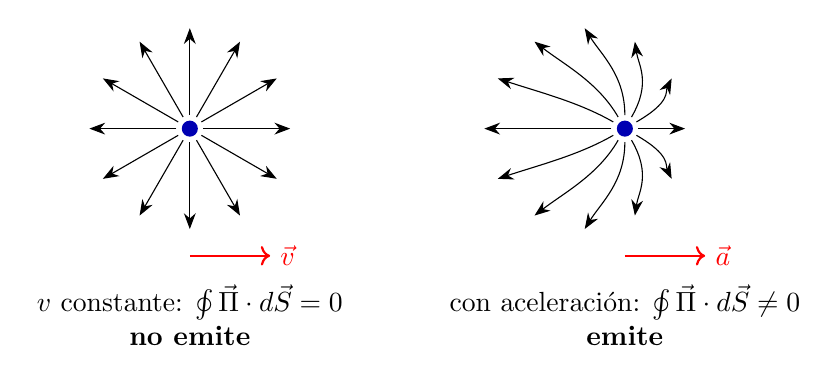
\begin{tikzpicture}[scale=0.85]
  % carga con v constante
  \begin{scope}
    \fill[blue!70!black] (0,0) circle (0.12);
    \foreach \a in {0,30,...,330}
      \draw[-{Stealth[length=2mm]}] (\a:0.2) -- (\a:1.5);
    \draw[->,thick,red] (0,-1.9) -- (1.2,-1.9) node[right]{$\vec v$};
    \node at (0,-2.6) {$v$ constante: $\oint\vec\Pi\cdot d\vec S=0$};
    \node at (0,-3.1) {\textbf{no emite}};
  \end{scope}
  % carga acelerada
  \begin{scope}[xshift=6.5cm]
    \fill[blue!70!black] (0,0) circle (0.12);
    \foreach \a in {0,30,...,330}
      \draw[-{Stealth[length=2mm]}] (\a:0.2) .. controls (\a:0.8) and ($(\a:1.1)+(-0.35,0)$) .. ($(\a:1.5)+(-0.6,0)$);
    \draw[->,thick,red] (0,-1.9) -- (1.2,-1.9) node[right]{$\vec a$};
    \node at (0,-2.6) {con aceleración: $\oint\vec\Pi\cdot d\vec S\neq0$};
    \node at (0,-3.1) {\textbf{emite}};
  \end{scope}
\end{tikzpicture}
\caption{Líneas de campo de una carga con velocidad constante (los campos se mueven con la carga) y de una carga acelerada (las líneas se curvan).}
\end{figure}
\end{document}
